\section{Introduction}

% Initial problem: Combining wearables and smart houses
\begin{frame}{Introduction}{Initial Problem}
\centering
Combining wearables and smart houses
\begin{figure}
  \subfloat{
    \includegraphics[width=0.48\textwidth]{images/wearables}
  }
  \subfloat{
    \includegraphics[width=0.48\textwidth]{images/smarthome}
  }
\end{figure}
\end{frame}

% Wearables body locations
\begin{frame}{Introduction}{Placement of wearables}
\centering
\begin{figure}
  \scalebox{0.8}{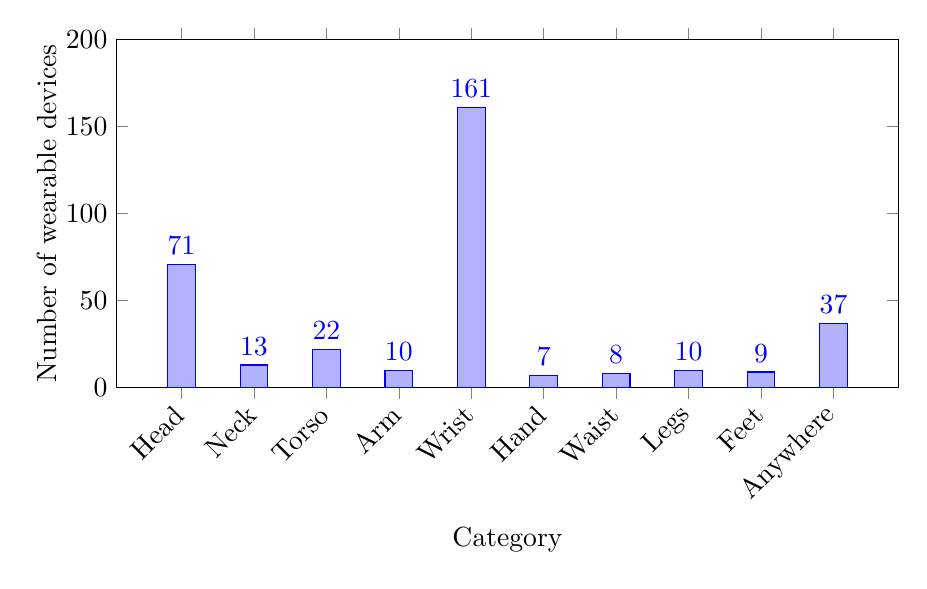
\begin{tikzpicture}
\begin{axis}[
    height=6cm,
    width=0.95\textwidth,
    xlabel={Category},
    xticklabel style={rotate=45, anchor=east, yshift=-0.5ex},
    ylabel={Number of wearable devices},
    yticklabel style={align=right,inner sep=0pt,xshift=-0.3em},
    nodes near coords align={vertical},
    nodes near coords,
    xtick=data,
    symbolic x coords={Head,Neck,Torso,Arm,Wrist,Hand,Waist,Legs,Feet,Anywhere},
    ybar,
    ymax=200,
    ymin=0,
    ]
    \addplot coordinates {(Head,71) (Neck,13) (Torso,22) (Arm,10) (Wrist,161) (Hand,7) (Waist,8) (Legs,10) (Feet,9) (Anywhere,37)};
\end{axis}
  

\end{tikzpicture}}
\end{figure}
{\tiny Data from vandrico.com}
\end{frame}

% Wearables applications
\begin{frame}{Introduction}{Applications of wearables}
\centering
\begin{figure}
  \scalebox{0.8}{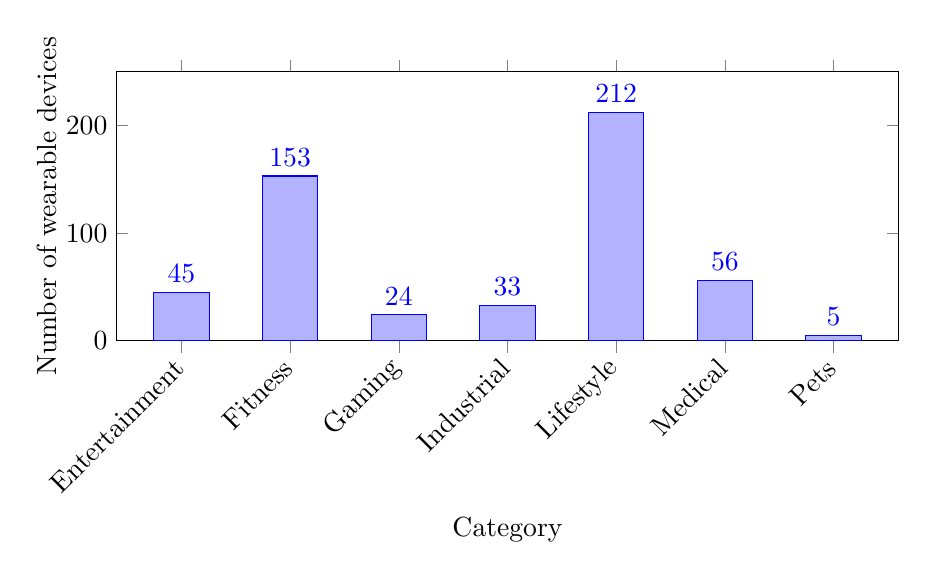
\begin{tikzpicture}
    \begin{axis}[
        height=5cm,
        width=0.95\textwidth,
        xlabel={Category},
        xticklabel style={rotate=45, anchor=east, yshift=-0.5ex},
        ylabel={Number of wearable devices},
        yticklabel style={align=right,inner sep=0pt,xshift=-0.3em},
        nodes near coords align={vertical},
        nodes near coords,
        xtick=data,
        symbolic x coords={Entertainment,Fitness,Gaming,Industrial,Lifestyle,Medical,Pets},
        ybar,
        ymax=250,
        ymin=0,
        bar width=20pt,
        ]
        \addplot coordinates {(Entertainment,45) (Fitness,153) (Gaming,24) (Industrial,33) (Lifestyle,212) (Medical,56) (Pets,5)};
    \end{axis}
\end{tikzpicture}}
\end{figure}
{\tiny Data from vandrico.com}
\end{frame}

% Wearables components
\begin{frame}{Introduction}{Components in wearables}
\centering
\begin{figure}
  \scalebox{0.8}{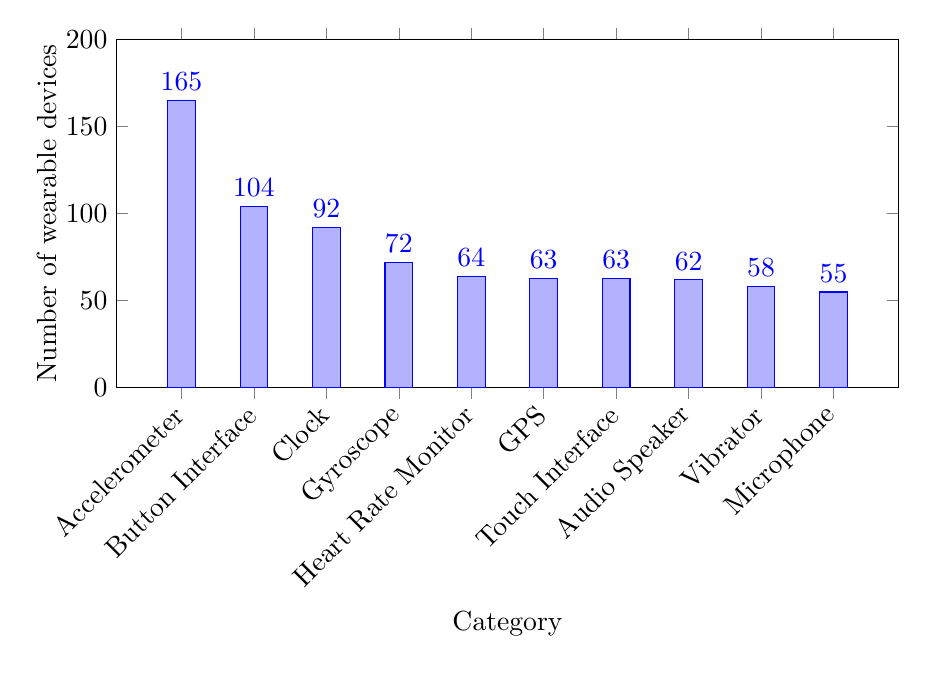
\begin{tikzpicture}
\begin{axis}[
    height=6cm,
    width=0.95\textwidth,
    xlabel={Category},
    xticklabel style={rotate=45, anchor=east, yshift=-0.5ex},
    ylabel={Number of wearable devices},
    yticklabel style={align=right,inner sep=0pt,xshift=-0.3em},
    nodes near coords align={vertical},
    nodes near coords,
    xtick=data,
    symbolic x coords={Accelerometer,Button Interface,Clock,Gyroscope,Heart Rate Monitor,GPS,Touch Interface,Audio Speaker,Vibrator,Microphone},
    ybar,
    ymax=200,
    ymin=0,
    ]
    \addplot coordinates {(Accelerometer,165) (Button Interface,104) (Clock,92) (Gyroscope,72) (Heart Rate Monitor,64) (GPS,63) (Touch Interface,63) (Audio Speaker,62) (Vibrator,58) (Microphone,55)};
\end{axis}
  

\end{tikzpicture}}
\end{figure}
{\tiny Data from vandrico.com}
\end{frame}

% Levels of home automation
\begin{frame}{Introduction}{Degrees of home automation}
\begin{itemize}
\item \textbf{Interactive systems}: Lowest degree of automation
\item \textbf{User defined rule systems}: Medium degree of automation
\item \textbf{Autonomous systems}: Highest degree of automation
\end{itemize}
\end{frame}

% Iron Man as a mental picture
\begin{frame}{Introduction}{Mental picture}
\centering
\begin{figure}
  \includegraphics[width=0.5\textwidth]{images/iron-man-1}
\end{figure}
{\tiny http://www.hypable.com/robert-downey-jr-salary-marvel/}
\begin{figure}
  \includegraphics[width=0.5\textwidth]{images/iron-man-2}
\end{figure}
{\tiny http://www.digitaltrends.com/home/mit-engineers-invented-cameraless-motion-tracker-home-automation/}
\end{frame}

% Reemo
\begin{frame}{Introduction}{Reemo}
\begin{itemize}
\item Requires a receiver placed near each smart device
\end{itemize}
\centering
\begin{figure}
  \includegraphics[width=0.7\textwidth]{images/reemo}
\end{figure}
{\tiny http://www.getreemo.com \\ https://www.youtube.com/watch?v=hSP5vqopgOQ}
\end{frame}

% Problem statement
\begin{frame}{Introduction}{Problem statement}
\begin{center}
How can wearables be utilized for home automation in a gesture driven solution?
\end{center}
\vfill
\hspace{0.1cm} {\color{black} \textbf{SCENARIO}}
\begin{tcolorbox}
\noindent
\begin{minipage}{0.40\textwidth}
\begin{enumerate}
  \item Point at the device
  \item Perform a gesture
\end{enumerate}
\end{minipage}
\hfill
\begin{minipage}{0.15\textwidth}
\centering
over
\end{minipage}
\hfill
\begin{minipage}{0.40\textwidth}
\begin{enumerate}
  \item Take up his smartphone
  \item Open up his smart hub application
  \item Find and select the device
  \item Find and select the action
\end{enumerate}
\end{minipage}
\end{tcolorbox}
\end{frame}

%%% Local Variables:
%%% mode: latex
%%% TeX-master: "../AAUsimpletheme"
%%% End:
